%
\begin{frame}
\frametitle{}
\begin{center}
  \textbf{\Large A SCE for the MOKP}
\end{center}
\end{frame}

%
\begin{frame}
\frametitle{A SCE for the MOKP}
As seen in previous sections
the SCE is easily applied to any optimization problem.
\\ \bigskip \pause
The fact that the MKP shares the same solution representation
as the MOKP allow us to use the same procedures
used on MKP.
\end{frame}

%
\begin{frame}
\frametitle{Non-dominated Sort}
Fitness computation for multi-objective solutions.
\medskip
\begin{columns}
\begin{column}{0.5\textwidth}  %%<--- here
  \begin{algorithmic}[1]
    \Function{NDSort}{$S:$ solution set}
      \State $i = 0$
      \While{ $S \neq \emptyset$ }
        \For{ $\sol{s} \in S$}
          %\State $D = \{ x \in X | \dom{x}{s}\}$
          \If{ $\nexists \sol{x} \in S : \dom{x}{s}$ }
            \State $o_s = i$
            \State $S = S - {x}$
          \EndIf
        \EndFor
        \State $i = i+1$
      \EndWhile
    \EndFunction
  \end{algorithmic}
\end{column}
\begin{column}{0.5\textwidth}
  \begin{figure}
    \centering
    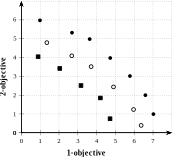
\includegraphics{img/pareto-sort}
  \end{figure}
\end{column}
\end{columns}
\end{frame}


%
\begin{frame}
\frametitle{Non-dominated Sort}
Fitness computation for multi-objective solutions.
\medskip

\end{frame}


% Schedule
\begin{frame}
\frametitle{Preliminary Computational Experiments}
Time and quality for bi-dimensional instances:
\begin{table}
\centering
{
\begin{tabular}{|cc|c|cc|}
 \hline
 { \bf Type}
 & {\bf n}
 & {\bf time (s) }
 & {\bf time (s)}
 & { \bf Hypervolume } \\ \hline
 A
 & 120
 & 479.5
 &  46.5
 &  97.0 \% \\ \hline
 B
 & 500
 & 503.6
 &  98.3
 &  98.6 \% \\ \hline
 C
 & 80
 & 559.1
 & 16.2
 & 94.4 \% \\ \hline
 D
 & 40
 & 462.0
 & 92.4
 & 97.2 \% \\ \hline
\end{tabular}
}
\end{table}
\end{frame}

\begin{frame}
\frametitle{Final Doctoral Schedule}
\begin{table}
\centering
{
\def\arraystretch{1.0}%
\fontsize{6.5pt}{1em}\selectfont
\begin{tabular}{|l|c:c:c|c:c:c:c|c:c:c:c|}
 \hline
  \multirow{3}{*}{\textbf{ \phantom{aaaa} Activities}}
  & \multicolumn{11}{c|}{\textbf{Weeks}} \\ \cline{2-12}
   & \multicolumn{3}{c|}{\textbf{ November }}
   & \multicolumn{4}{c|}{\textbf{December}}
   & \multicolumn{4}{c|}{\textbf{January}} \\ \cline{2-12}
  & \;2º\; & 3º & 4º & 1º & 2º & 3º & 4º & 1º & 2º & 3º & 4º \\ \hline
 Literature review
  & $\bbt$ & $\bbt$ & $\bbt$ & & & & & & & & \\ \hline
 Implementation and adjustments
  & $\bbt$ & $\bbt$ & $\bbt$ & $\bbt$ & & & & & & & \\ \hline
 Computational experiments
  & & & $\bbt$ & $\bbt$ & $\bbt$ & & & & & & \\ \hline
 CEC Paper writing
  & & & & & & $\bbt$ & $\bbt$ & $\bbt$ & & & \\ \hline
 CEC Paper submission
  & & & & & & & & & $\bbt$ & & \\ \hline
 Thesis writing
  & & & & $\bbt$ & $\bbt$ & $\bbt$ & $\bbt$ & $\bbt$ & $\bbt$ & $\bbt$ & \\ \hline
\end{tabular}
}
\end{table}
\end{frame}
